\documentclass{beamer}
\begin{document}
\title{Introduction to the J Programming Language}   
\author{Wayne Chang}
\date{\today} 

\frame{\titlepage} 

\frame{\frametitle{Table of contents}\tableofcontents} 


\section{History} 
\subsection{What is J?}
\frame{\frametitle{What is J?} 

J is a programming language that is:
\begin{itemize}
\item Functional
  \begin{itemize}
  \item Higher-order functions
  \item Immutable Data
  \end{itemize}
\item Dynamic
  \begin{itemize}
  \item Dynamically typed
  \item Parsing tightly coupled with evaluation
  \end{itemize}
\item Array-based
  \begin{itemize}
  \item Arrays (matrices) are first-class citizens
  \item Operators can all operate in higher dimensions
  \end{itemize}
\item Tacit
  \begin{itemize}
  \item Most operations are function composition
  \item Higher-order function everywhere
  \item Learn where parameters go
  \end{itemize}
\end{itemize}
}

\subsection{Why J?}
\frame{\frametitle{Why J?} 
  \begin{itemize}
  \item Operations on Matrices
  \item Mathematical and Statistical Programming
  \item Signal Processing
  \item Examples
    \begin{itemize}
      \item Financial and Insurance Risk Calculations
      \item Network Flow Analysis
      \item Polling Institutions
      \item Econometrics
    \end{itemize}
  \end{itemize}
}

\subsection{Spiritual Successor to APL}
\frame{\frametitle{Spiritual Successor to APL}
\begin{itemize}
\item Stands for ``A Programming Language'' 
\item Developed in the 1960s by Kenneth E. Iverson
\item Not a Von Neumann language (isomorph of the machine)
\item Conway's Game of Life in one line of APL:
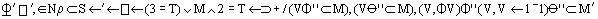
\includegraphics[scale=0.5]{apllife}
\item J was developed in the early 1990's by Ken Iverson and Roger Hui
\end{itemize} 
}

\section{The Language} 
\subsection{Terminology and Examples}
\frame{\frametitle{Terminology: Nouns, Verbs, Adverbs, Operators}
\begin{itemize}
\item Right-to-left evaluation
\item Nouns are data like 100, ``hello, world!'', and 1.333
\item Verbs are ordinary functions like $+$ or $-$
\item Adverbs and operators are functions that compute functions from functions
\end{itemize}
}

\frame{\frametitle{Monads and Dyads}
\begin{itemize}
\item Monads are verbs that take one argument on the right: $*: 4$
\item Dyads are verbs that take one argument each side: $2 + 2$
\item The same symbol has multiple meanings depending on the context
\end{itemize}
\begin{tabular}{|c|c|c|}
\hline
\textbf{Symbol} & \textbf{Monadic} & \textbf{Dyadic} \\
\hline
+ & Conjugate & Plus \\
\hline
$-$ & Negate & Minus \\
\hline
$<.$ & Integral Floor & Lesser of \\
\hline
$|$ & Magnitude & Residue \\
\hline
\end{tabular}
}


\frame{\frametitle{Arrays and Boxes}
\begin{itemize}
  \item Different from arrays in other programming languages.
  \item A table is a 2-dimensional array.
  \item Arrays have rank and shape.
  \item Cue array example: shape, tally \#, index of/integers (i.), join (,), from (\{), match ($-:$)
  \item Cue box example: open ($>$), box ($<$)
\end{itemize}
}

\frame{\frametitle{Examples}
\begin{itemize}
  \item sum, product (introducing the / operator)
  \item vector magnitude (introducting bonding with \&)
  \item taxes and percentages (introducing hooks)
  \item mean (introducing forks)
  \item 1D kernel convolution
  \item stateless FizzBuzz
  \item various euler problems
  \item introspection with 5!:4, 7!:2, 6!:2
\end{itemize}
}

\end{document}

